\documentclass[titlepage, 11pt]{article}
\title{Practical Machine Learning: Final project }
\author{Mathias Mellemstuen}
\date{16 December 2021}
\usepackage{times}
\renewcommand{\baselinestretch}{1.5}

\usepackage[margin=1.0in]{geometry}
\usepackage{listings}
\usepackage{color}

\definecolor{dkgreen}{rgb}{0,0.6,0}
\definecolor{gray}{rgb}{0.5,0.5,0.5}
\definecolor{mauve}{rgb}{0.58,0,0.82}

\usepackage{graphicx}
\graphicspath{./}

\lstset{frame=tb,
	aboveskip=3mm,
	belowskip=3mm,
	showstringspaces=false,
	columns=flexible,
	basicstyle={\small\ttfamily},
	numbers=none,
	numberstyle=\tiny\color{gray},
	keywordstyle=\color{blue},
	commentstyle=\color{dkgreen},
	stringstyle=\color{mauve},
	breaklines=true,
	breakatwhitespace=true,
	tabsize=3
}

\begin{document}
    \maketitle

    \section{Task 1: Two-layer perceptron}
    This was the result after running the code I created for this task. If you look at the output text below, you will see that when the learning rate is increasing, the epochs is decreasing. This is excepted. \newline The text below is the console output from the python script.
    \begin{lstlisting}
        Learning rate of 0.05 results in number of epochs of 44832
        Learning rate of 0.1 results in number of epochs of 22384
        Learning rate of 0.15 results in number of epochs of 14896
        Learning rate of 0.2 results in number of epochs of 11168
        Learning rate of 0.25 results in number of epochs of 8912
        Learning rate of 0.3 results in number of epochs of 7424
        Learning rate of 0.35 results in number of epochs of 6352
        Learning rate of 0.4 results in number of epochs of 5552
        Learning rate of 0.45 results in number of epochs of 4928
        Learning rate of 0.5 results in number of epochs of 4432
    \end{lstlisting}
    \lstset{frame=tb,
        language=Python,
        aboveskip=3mm,
        belowskip=3mm,
        showstringspaces=false,
        columns=flexible,
        basicstyle={\small\ttfamily},
        numbers=none,
        numberstyle=\tiny\color{gray},
        keywordstyle=\color{blue},
        commentstyle=\color{dkgreen},
        stringstyle=\color{mauve},
        breaklines=true,
        breakatwhitespace=true,
        tabsize=3
    }

    \begin{center}
        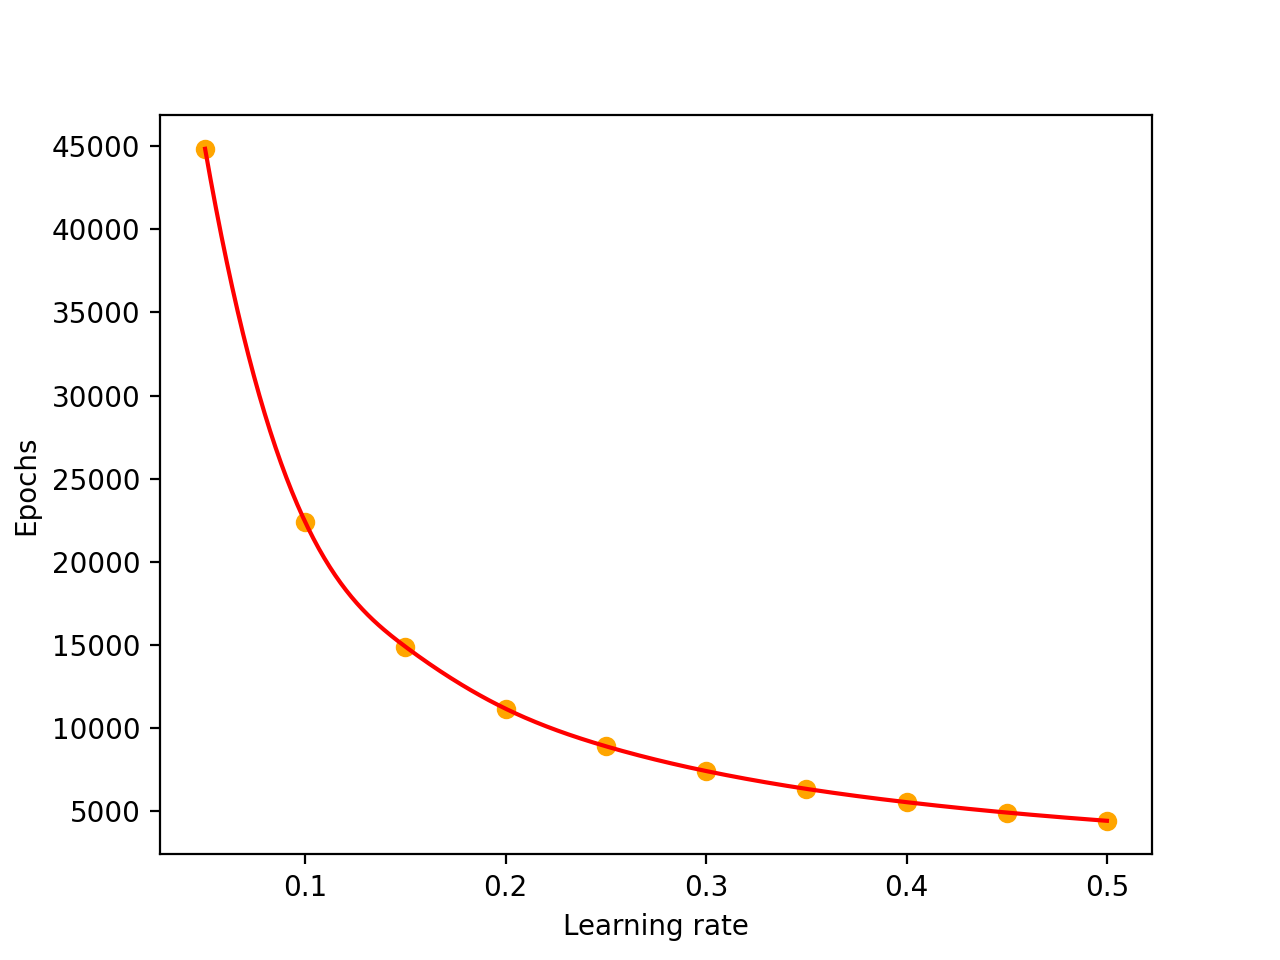
\includegraphics[]{Task1.png}
    \end{center}
    It becomes much clearer when plotting it. It does significantly less epochs when the learning rate is at 0,5 compared to 0,05. This result is very excepted. The neural network will learn more agressivly if the learning rate is higher. When the learning rate is higher, the weights will be allowed to be adjusted more at each epoch. The weights will then reach a satisfied value much quicker because of this. The learning rate is still a hyperparameter that needs tuning. That is because a lower learning rate will allow more precise adjustments of the weights, thus running a lot longer with more epochs. 
    \section{Task 2: Multiple Depots Vehicle Routing Problem}
\end{document}